\subsection{Sequenzdiagramme}

\subsubsection{Sensorfehler/Warnmodus}

\begin{figure}[H]
	\centering
	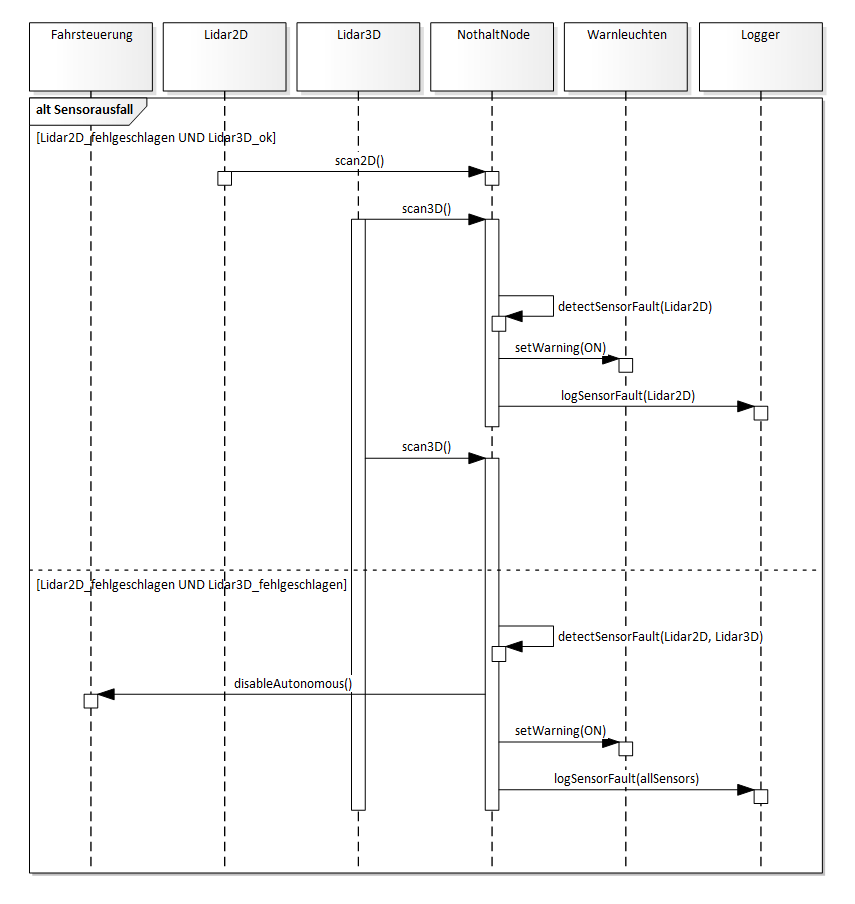
\includegraphics[width = \imglarge]{images/Seq4_Sensorfehler_Warnmodus.png}
	\caption{Sequenzdiagramm „Sensorfehler/Warnmodus“}
	\label{fig:sequenz_sensorfehler_warnmodus}
\end{figure}

\quad Das Sequenzdiagramm beschreibt das Verhalten des Systems, wenn einer oder mehrere Lidarsensoren fehlschlagen. Die Verarbeitung unterscheidet dabei klar zwischen dem Ausfall eines einzelnen Sensors und dem gleichzeitigen Ausfall beider Sensorquellen.

\quad Das Ziel dieses Modells ist es, den Übergang in den Warnmodus nachvollziehbar zu spezifizieren, ohne einen \ac{Hardstop} 
auszulösen, solange zumindest eine valide Sensorquelle zur Verfügung steht.

\subsubsection*{Ablaufbeschreibung}

\paragraph{1. Zyklische Sensordatenerfassung} 
\quad Sowohl der 2D-Lidar als auch der 3D-Lidar senden kontinuierlich Sensordaten an die Nothalt-Node:
\begin{itemize}
    \item scan2D()
    \item scan3D()
\end{itemize}

\quad Diese Sensordaten bilden die Grundlage für die weitere Verarbeitung in der Entscheidungslogik.

\paragraph{2. Alternativer Entscheidungsblock (alt): Sensorfehler}
\textbf{Fall A – 2D-Lidar ausgefallen, 3D-Lidar funktionsfähig}

\begin{description}
    \item[\texttt{[Lidar2D\_fehlgeschlagen UND Lidar3D\_ok]}]
\end{description}

\quad Ablauf:
\begin{enumerate}
    \item Der 3D-Lidar liefert weiterhin scan3D() Daten.
    \item Die Nothalt-Node erkennt den Fehler:
    \begin{itemize}
        \item detectSensorFault(Lidar2D)
    \end{itemize}
    \item Das System aktiviert die Warnsignale:
    \begin{itemize}
        \item setWarning(ON)
    \end{itemize}
    \item Der Logger dokumentiert den Fehler:
    \begin{itemize}
        \item logSensorFault(Lidar2D)
    \end{itemize}
\end{enumerate}

\quad Interpretation:  
Der autonome Betrieb darf vorsichtig weiterlaufen, da der 3D-Sensor als redundante Sicherheitsquelle weiterhin korrekt arbeitet.

\vspace{1em}

\textbf{Fall B – Beide Sensoren fehlerhaft}

\begin{description}
    \item[\texttt{[Lidar2D\_fehlgeschlagen UND Lidar3D\_fehlgeschlagen]}]
\end{description}

\quad Ablauf:
\begin{enumerate}
    \item Die Nothalt-Node erkennt den vollständigen Ausfall:
    \begin{itemize}
        \item detectSensorFault(Lidar2D, Lidar3D)
    \end{itemize}
    \item Aktivieren der Warnsignale:
    \begin{itemize}
        \item setWarning(ON)
    \end{itemize}
    \item Protokollierung des kombinierten Fehlers:
    \begin{itemize}
        \item logSensorFault(allSensors)
    \end{itemize}
    \item Die Fahrsteuerung wird informiert:
    \begin{itemize}
        \item disableAutonomous()
    \end{itemize}
\end{enumerate}

\quad Interpretation:  
Das Fahrzeug darf nicht mehr autonom bewegt werden. Im Zustandsdiagramm führt dies zum \ac{Warnmodus}.

\paragraph{3. Bedeutung im Gesamtsystem}

\quad Der Ablauf stellt sicher, dass:
\begin{itemize}
    \item nicht sofort \ac{Hardstop} ausgelöst wird, wenn nur ein Sensor betroffen ist
    \item Redundanz genutzt wird, solange mindestens ein Sensor valide Daten liefert
    \item Warnmodus aktiviert wird, sobald keinerlei sichere Messdaten mehr vorliegen
    \item stets ein definierter sicherer Zustand erreicht wird
    \item Fehler systematisch dokumentiert werden
\end{itemize}

\paragraph{Zusammenfassung}

\quad Das Sequenzdiagramm demonstriert:
\begin{enumerate}
    \item die redundante Sensorverarbeitung,
    \item die klare Unterscheidung zwischen teilweisem und vollständigem Sensorfehler,
    \item die Aktivierung des Warnmodus statt eines sofortigen \ac{Hardstop},
    \item die Weitergabe der Statusinformationen an Warnleuchten und Logger,
    \item die sichere Deaktivierung des autonomen Fahrbetriebs bei Totalausfall.
\end{enumerate}

\vspace{1em}

% ------------------------------------------------------
\subsubsection{Softstop-Sequenz}
\begin{figure}[H]
    \centering
    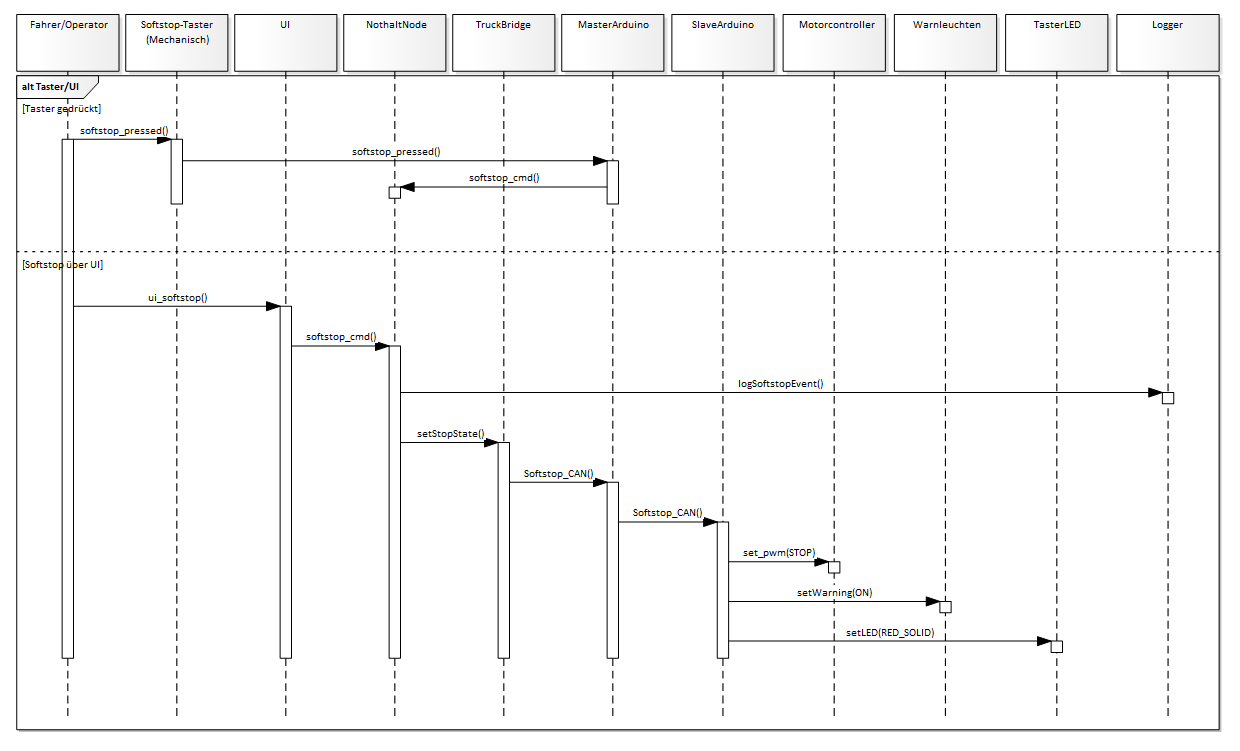
\includegraphics[width = \imglarge]{images/Seq2_Softstop_manuell.png}
    \caption{Sequenzdiagramm „Softstop"}
    \label{fig:sequenz_softstop}
\end{figure}

\quad Das Sequenzdiagramm zeigt den Ablauf eines \ac{Softstop}s, der entweder durch den mechanischen \ac{Softstop}-Taster oder über die Benutzeroberfläche (UI) ausgelöst wird.  
Der \ac{Softstop} stellt einen kontrollierten, nicht systemverriegelnden Stopp dar und hat geringere 
Priorität als \ac{Hardstop} und \ac{E-Stop}. Dennoch führt er zu einer sofortigen Reduktion der Geschwindigkeit bzw. einem Anhalten des Fahrzeugs.
Die Darstellung nutzt einen alt-Block zur Unterscheidung beider Auslösewege.

\subsubsection*{Ablaufbeschreibung}

\paragraph{1. Alternativer Auslöser: Taster oder UI}

\textbf{Fall A – Softstop über mechanischen Taster}

\begin{description}
    \item[\texttt{[Taster gedrückt]}]
\end{description}

Ablauf:
\begin{enumerate}
    \item Der Fahrer betätigt den mechanischen Softstop-Taster:
    \begin{itemize}
        \item softstop\_pressed()
    \end{itemize}
    \item Das UI zeigt die Aktivierung an (sofern gekoppelt).
    \item Die Nothalt-Node empfängt das Tastensignal:
    \begin{itemize}
        \item softstop\_cmd()
    \end{itemize}
    \item Die interne State-Machine setzt Softstop als aktiven Zustand.
\end{enumerate}

\textbf{Fall B – Softstop über UI}

\begin{description}
    \item[\texttt{[Softstop über UI]}]
\end{description}

Ablauf:
\begin{enumerate}
    \item Softstop wird über das UI ausgelöst:
    \begin{itemize}
        \item ui\_softstop()
    \end{itemize}
    \item UI sendet den Befehl an die Nothalt-Node:
    \begin{itemize}
        \item softstop\_cmd()
    \end{itemize}
    \item Die Nothalt-Node setzt den Softstop-Zustand:
    \begin{itemize}
        \item setStopState()
    \end{itemize}
    \item Weitergabe über CAN:
    \begin{itemize}
        \item Softstop\_CAN()
    \end{itemize}
    \item Weitergabe an MasterArduino:
    \begin{itemize}
        \item Softstop\_CAN()
    \end{itemize}
    \item Sicherungsaktionen:
    \begin{itemize}
        \item set\_pwm(STOP)
        \item setWarning(ON)
        \item setLED(RED\_SOLID)
    \end{itemize}
    \item Logging:
    \begin{itemize}
        \item logSoftstopEvent()
    \end{itemize}
\end{enumerate}

\paragraph{2. Wirkungskette des Softstops}

\quad Der Ablauf macht klar:
\begin{itemize}
    \item \ac{Softstop} beeinflusst direkt die Aktorik (PWM STOP).
    \item \ac{Softstop} aktiviert Warnleuchten, aber nicht den Warnmodus.
    \item \ac{Softstop} aktiviert die Taster-LED, aber nicht die Verriegelung (wie beim \ac{Hardstop}).
    \item \ac{Softstop} wird vollständig über ROS → CAN → Arduino → Motorcontroller propagiert.
\end{itemize}

\paragraph{3. Protokollierung}

\quad Das Logging sorgt für:
\begin{itemize}
    \item Nachvollziehbarkeit bei Tests
    \item Diagnose von Fehlbedienungen
    \item Analyse in der Sicherheitstechnik
\end{itemize}

% ------------------------------------------------------
\subsubsection{E-Stop-Sequenz}
\begin{figure}[H]
	\centering
	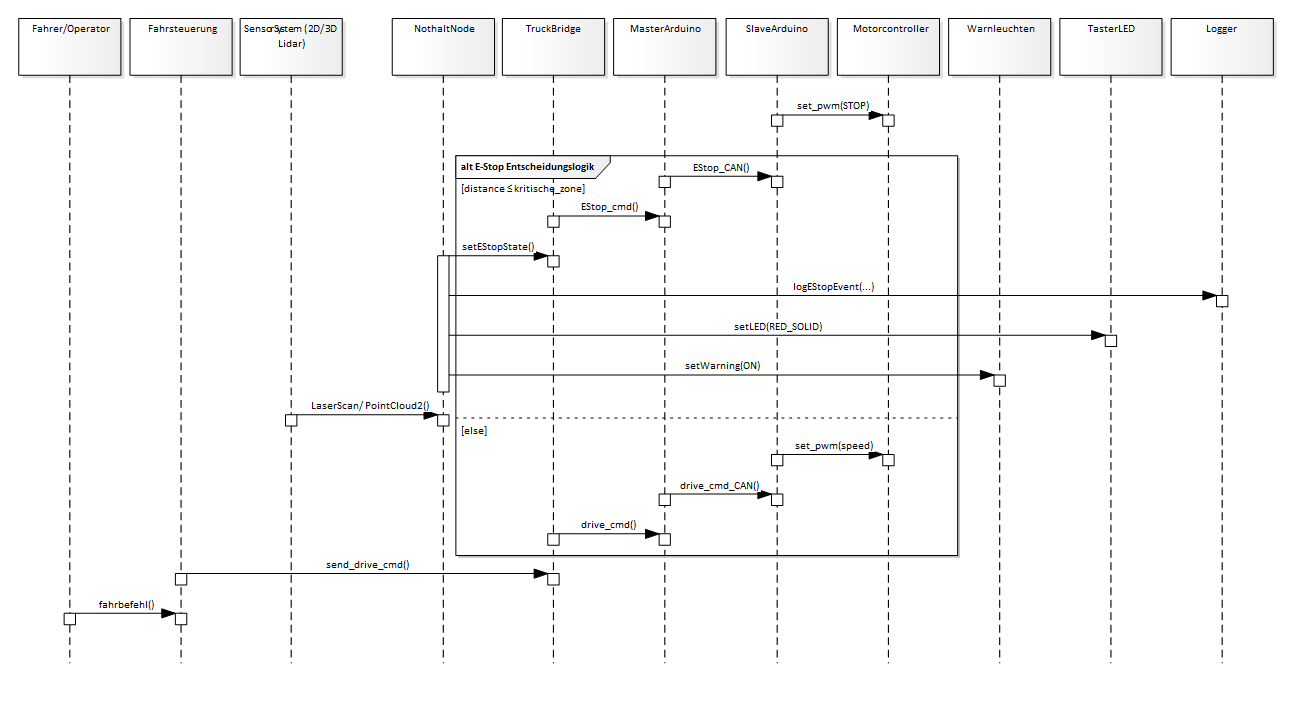
\includegraphics[width = \imglarge]{images/Seq1_EmergencyStop_automatisch.png}
	\caption{Sequenzdiagramm „E-Stop“}
	\label{fig:sequenz_estop}
\end{figure}

\subsubsection*{Ablaufbeschreibung}

\paragraph{1. Sensorerfassung der Umgebung}

\quad Das Sensorsystem übermittelt kontinuierlich Umgebungsdaten an die Nothalt-Node:
\begin{itemize}
    \item LaserScan()
    \item PointCloud2()
\end{itemize}

\paragraph{2. \ac{E-Stop} Entscheidungslogik}

\quad Die Nothalt-Node verarbeitet die Sensordaten in einem alt-Block:

\textbf{Fall A – Hindernis in kritischer Zone}

Bedingung:
\begin{description}
    \item[\texttt{[distance <= kritische\_zone]}]
\end{description}

Ablauf:
\begin{enumerate}
    \item setEStopState()
    \item EStop\_cmd() an TruckBridge
    \item EStop\_CAN() an MasterArduino
    \item MasterArduino:
    \begin{itemize}
        \item setLED(RED\_SOLID)
        \item setWarning(ON)
        \item logEStopEvent(...)
    \end{itemize}
    \item set\_pwm(STOP) an SlaveArduino
    \item Motorcontroller stoppt sofort
\end{enumerate}

\textbf{Fall B – Kein Hindernis in kritischer Zone}

Bedingung:
\begin{description}
    \item[\texttt{[distance > kritische\_zone]}]
\end{description}

Ablauf:
\begin{enumerate}
    \item drive\_cmd()
    \item drive\_cmd\_CAN()
    \item set\_pwm(speed)
\end{enumerate}

\paragraph{3. Fahrbefehle des Operators}

\quad Fahrzyklus:
\begin{itemize}
    \item fahrbefehl() vom Operator
    \item send\_drive\_cmd() an Nothalt-Node
\end{itemize}

\paragraph{4. Logging des E-Stop-Ereignisses}

\quad Der Logger speichert:
\begin{itemize}
    \item Zeitpunkt
    \item Sensorwerte
    \item Auslöser
    \item Fahrzeugstatus
    \item Aktorreaktionen
\end{itemize}

\paragraph{Zusammenfassung}

\quad Das Sequenzdiagramm zeigt:
\begin{enumerate}
    \item automatischer E-Stop durch kritische Zone
    \item vollständige Sicherheitskette (Master/Slave/Controller)
    \item sofortiger Motorstopp
    \item Aktivierung der Warnsignale
    \item Protokollierung
\end{enumerate}

% ------------------------------------------------------
\subsubsection{Quittierung \& Kriechmodus}
\begin{figure}[H]
	\centering
	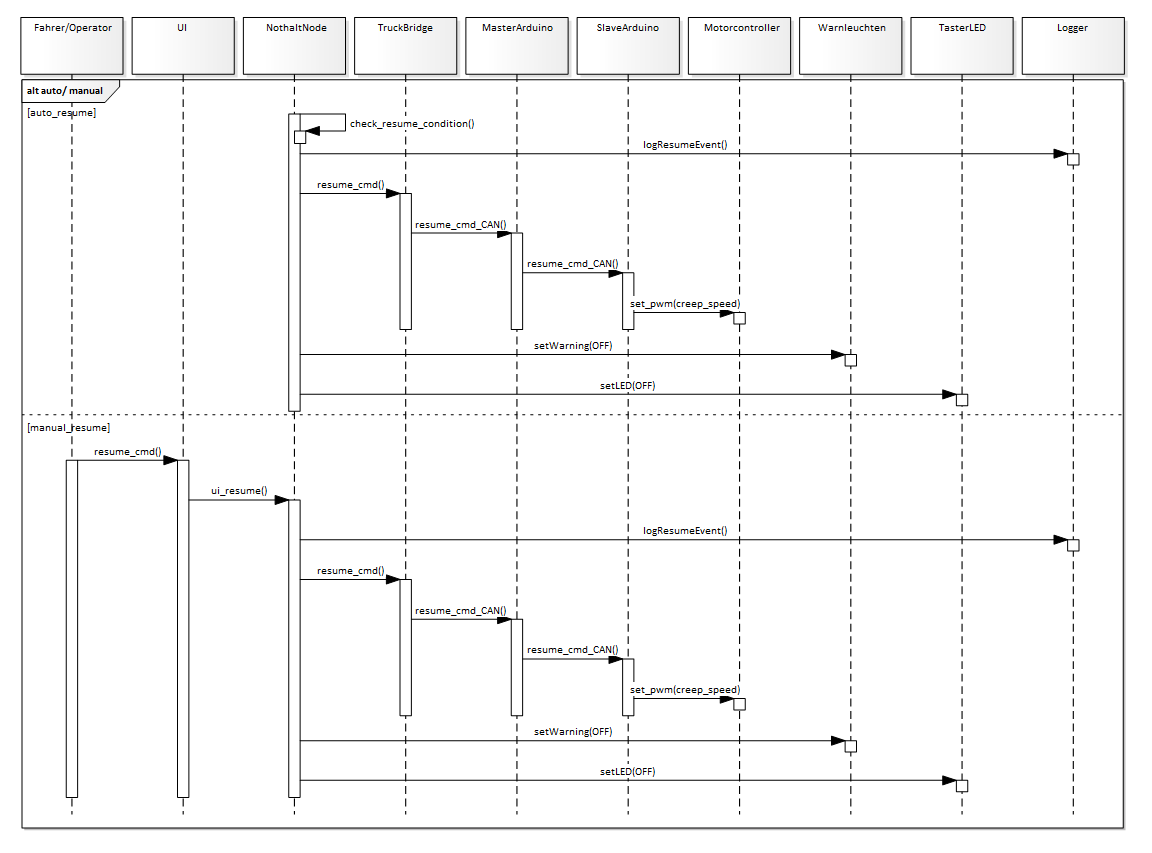
\includegraphics[width = \imglarge]{images/Seq3_Freigabe_Kriechmodus.png}
	\caption{Sequenzdiagramm „Quittierung \& Kriechmodus“}
	\label{fig:sequenz_quittierung_kriechmodus}
\end{figure}
\quad Das Sequenzdiagramm zeigt den Ablauf, mit dem das Fahrzeug den Fahrbetrieb nach einem Softstop oder E-Stop wieder aufnehmen kann. Die Wiederaufnahme kann automatisch erfolgen, wenn alle Sicherheitsbedingungen erfüllt sind, oder manuell durch den Operator.

\quad Das Diagramm unterscheidet:
\begin{itemize}
    \item Auto-Resume
    \item Manual-Resume
\end{itemize}

\paragraph{Fall A – Auto-Resume}

Bedingung:
\begin{description}
    \item[\texttt{[auto\_resume]}]
\end{description}

Ablauf:
\begin{enumerate}
    \item check\_resume\_condition()
    \item resume\_cmd()
    \item resume\_cmd\_CAN()
    \item MasterArduino:
    \begin{itemize}
        \item set\_pwm(creep\_speed)
        \item setWarning(OFF)
        \item setLED(OFF)
    \end{itemize}
    \item logResumeEvent()
\end{enumerate}

\paragraph{Fall B – Manual-Resume}

Bedingung:
\begin{description}
    \item[\texttt{[manual\_resume]}]
\end{description}

Ablauf:
\begin{enumerate}
    \item resume\_cmd() über UI
    \item resume\_cmd\_CAN()
    \item MasterArduino:
    \begin{itemize}
        \item set\_pwm(creep\_speed)
        \item setWarning(OFF)
        \item setLED(OFF)
    \end{itemize}
    \item logResumeEvent()
\end{enumerate}

\paragraph{Kriechmodus}

\quad Beide Wege führen zu:
\begin{itemize}
    \item set\_pwm(creep\_speed)
\end{itemize}

\quad Damit entsteht ein sicherer, langsamer Start:
\begin{itemize}
    \item minimale Geschwindigkeit
    \item volle Operator-Kontrolle
    \item geeignet für enges Rangieren
\end{itemize}

\paragraph{Systemwirkungen und Konsistenz}

\quad Das Sequenzdiagramm ist konsistent mit:
\begin{itemize}
    \item Zustandsdiagrammen (Softstop/E-Stop → Resume → Kriechmodus)
    \item Aktivitätsdiagrammen
    \item Requirements (FR-SOFTSTOP, FR-ESTOP, FR-Kriechmodus, FR-INT-CAN)
    \item Sicherheitspriorisierung
\end{itemize}

\paragraph{Zusammenfassung}

\quad Dieses Sequenzdiagramm bildet alle relevanten Aspekte des Wiederanfahrens ab:
\begin{enumerate}
    \item automatische Wiederaufnahme
    \item manuelle Wiederaufnahme
    \item vollständige Weitergabe über ROS → CAN → Arduino
    \item sichere Freigabe in den Kriechmodus
    \item Abschalten der Warnsignale
    \item Protokollierung aller Resume-Ereignisse
\end{enumerate}

